\documentclass[12pt]{article}
\usepackage[top=1in, bottom=1in, left=1in, right=1in]{geometry}

\usepackage{setspace}
\onehalfspacing

\usepackage{amssymb}
%% The amsthm package provides extended theorem environments
\usepackage{amsthm}
\usepackage{epsfig}
\usepackage{times}
\renewcommand{\ttdefault}{cmtt}
\usepackage{amsmath}
\usepackage{graphicx} % for graphics files
\usepackage{tabu}

% Draw figures yourself
\usepackage{tikz} 

% writing elements
%\usepackage{mhchem}

\usepackage{paralist}

% The float package HAS to load before hyperref
\usepackage{float} % for psuedocode formatting
\usepackage{xspace}

% from Denovo Methods Manual
\usepackage{mathrsfs}
\usepackage[mathcal]{euscript}
\usepackage{color}
\usepackage{array}
\usepackage{cite}
% \usepackage{c++}
% \usepackage{tmadd,tmath}
\usepackage{subcaption}
\usepackage{booktabs}
\usepackage{algorithm}
\usepackage{algpseudocode}

\usepackage[pdftex]{hyperref}
\usepackage[parfill]{parskip}

% math syntax
\newcommand{\nth}{n\ensuremath{^{\text{th}}} }
\newcommand{\ve}[1]{\ensuremath{\mathbf{#1}}}
\newcommand{\Macro}{\ensuremath{\Sigma}}
\newcommand{\rvec}{\ensuremath{\vec{r}}}
\newcommand{\vecr}{\ensuremath{\vec{r}}}
\newcommand{\omvec}{\ensuremath{\hat{\Omega}}}
\newcommand{\vOmega}{\ensuremath{\hat{\Omega}}}
\newcommand{\even}{\ensuremath{\phi^g}}
\newcommand{\odd}{\ensuremath{\vartheta^g}}
\newcommand{\evenp}{\ensuremath{\phi^{g'}}}
\newcommand{\oddp}{\ensuremath{\vartheta^{g'}}}
\newcommand{\Sn}{\ensuremath{S_N} }
\newcommand{\Ye}[2]{\ensuremath{Y^e_{#1}(\vOmega_#2)}}
\newcommand{\sigg}[1]{\ensuremath{\Macro^{gg'}_{s\,#1}}}
\newcommand{\psig}{\ensuremath{\psi^g}}
\newcommand{\Di}{\ensuremath{\Delta_i}}
\newcommand{\Dj}{\ensuremath{\Delta_j}}
\newcommand{\Dk}{\ensuremath{\Delta_k}}
%---------------------------------------------------------------------------
%---------------------------------------------------------------------------
\begin{document}
\begin{center}
{\bf NE 155/255, Fall 2019 \\
Spatial Discretization\\
October 14, 2019}
\end{center}

\setlength{\unitlength}{1in}
\begin{picture}(6,.1) 
\put(0,0) {\line(1,0){6.25}}         
\end{picture}

So far we've dealt with
\begin{compactitem}
\item Discretization of \textit{energy} using the multigroup approximation, where we assume group-integrated values. 
\item \textit{Expanding sources}, in particular scattering, in spherical harmonics -- which we reduce to Legendre Polynomials in the case of azimuthal symmetry
\item Discretization of \textit{angle}, one of
  \begin{compactitem}
  \item $S_N$: get solutions along specific angle sets (quadrature points), use corresponding quadrature weights to integrate over angle
  \item $P_N$: expand the angular flux in spherical harmonics (which we only do in 1-D, so Legendre polynomials in practice) and solve a set of coupled equations for each expansion term
  \item $SP_N$: take the 1-D $P_N$ equations and transform them to 3-D by replacing the 1-D diffusion operators with the 3-D diffusion operator and replacing the derivatives at the boundary with the outward normal derivatives
  \end{compactitem}
\end{compactitem}

When we do all of this we get $g=0,\dots,G-1$ equations in energy, and some number of equations in angle that depends on which approach we take. However, we still have one major item to deal with: space.

\section*{Space}
(Largely from Evans; some from Vuj\'ic, Lewis and Miller)

There are \textit{many} spatial discretization choices out there. What you choose can depend on the geometry and physical properties, as well as if you're using Cartesian or curvilinear formulations. Fundamentally, we can characterize the differencing schemes in a few ways
\begin{compactitem}
\item Cell balance, which includes
  \begin{compactitem}
  \item Finite Difference Method (FDM) -- using point value solution	
  \item Finite Volume Method (FVM) -- using cell-averaged value solution
  \end{compactitem}	
\item Finite element (FEM) -- using basis function for expansion:	
  \begin{compactitem}
  \item Piecewise linear: hat functions	
  \item Piecewise quadratic or cubic basis functions	
  \item Piecewise higher order Gauss-Legendre polynomials	
  \end{compactitem}
\item Spectral and Pseudo Spectral Methods -- using orthogonal global series as the basis function:	
  \begin{compactitem}
  \item Fourier series	
  \item Bessel, Chebyshev, Legendre series
  \end{compactitem}
\end{compactitem}

We'll talk about cell balance and finite element methods; in nuclear engineering we have specific versions of these. For example, Denovo, the 3-D Cartesian mesh deterministic code from ORNL, offers these choices:
\begin{compactitem}
\item Simplified P$_N$: finite volume 
\item Discrete ordinates: weighted diamond difference (WDD) without flux fixup is equivalent to a Crank-Nicolson method; cell balance.
\item Discrete ordinates: weighted diamond difference with flux fixup to zero (WDD-FF)  is a nonlinear method; cell balance 
\item Discrete ordinates: theta weighted diamond difference (TWD)  is a nonlinear method; cell balance
\item Discrete ordinates: linear discontinuous (LD) is a Galerkin method formed from the basis set $\{1,x,y,z\}$; FEM 
\item Discrete ordinates: bilinear discontinuous (BLD) in 2-D; FEM
\item Discrete ordinates: trilinear discontinuous (TLD) is a Galerkin method formed from the basis set $\{1,x,y,z,xy,yz,xz,xyz\}$ and maintains the asymptotic diffusion limit on the grid used in Denovo; FEM
\item Discrete ordinates: step characteristics (SC) in 2- or 3-D does not produce negative fluxes and does not have oscillatory behavior; can be written as a cell balance or finite element scheme
\end{compactitem}
The WDD, WDD-FF, TWD, LD, BLD, and TLD schemes are all second-order, and the SC scheme is first-order.  

\hrulefill

LANL's PARTIS$_N$ has similar choices, but their new Capsaicin code has unstructured mesh and uses Discontinuous Finite Element Method (DFEM): Linear, Bars, Triangles, Quadrilaterals, Polygons. They also have an ability to deal with non-convex meshes using Continuous FEM. Finally, they have structured meshes in 3-D with DD and LD.

INL's Rattle$S_N$ake uses finite element methods for unstructured higher-order
meshes as well, and has capabilities for both discontinuous and continuous Galerkin.

We'll use the diagram in \ref{fig:spatial_mesh} to think through our discretization schemes.

\begin{figure}[!htb]
\centering
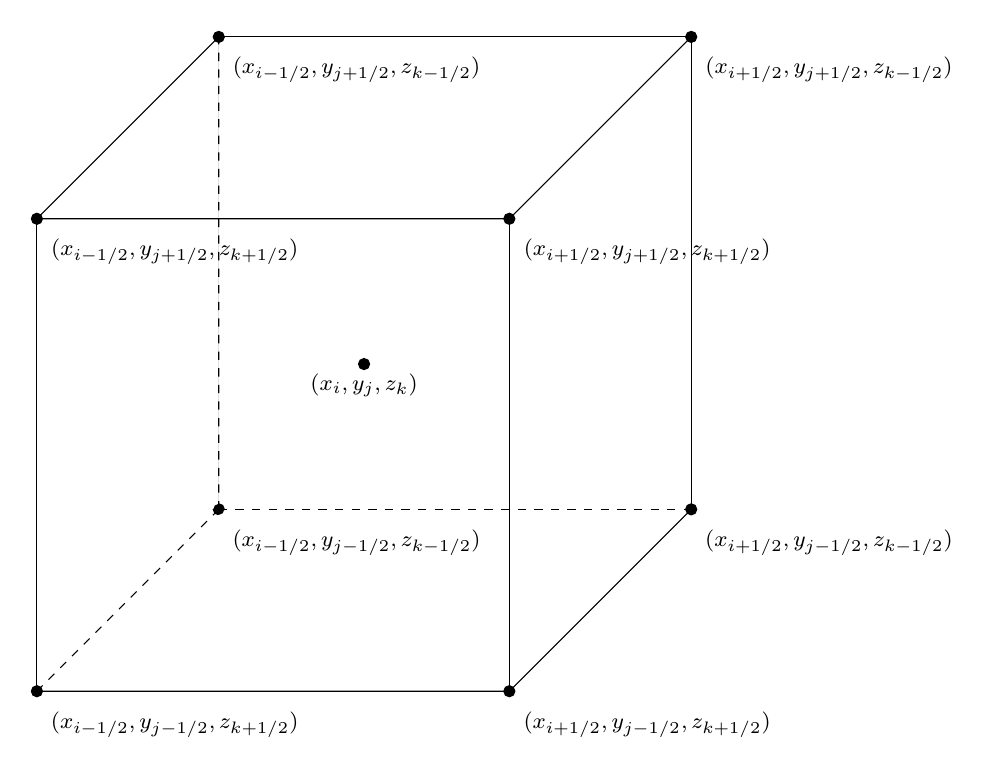
\begin{tikzpicture}
\filldraw (xyz cs:x=-3,y=-3,z=3) circle (2pt) node {} -- 
          (xyz cs:x=3,y=-3,z=3) circle (2pt) node {};
\node[fill,circle,inner sep=0pt, minimum size = 2pt,
      label={[shift={(1.75,-0.75)}]
      \footnotesize$(x_{i-1/2}, y_{j-1/2}, z_{k+1/2})$}] 
      at (xyz cs:x=-3,y=-3,z=3) {};
\node[fill,circle,inner sep=0pt, minimum size = 2pt,
      label={[shift={(1.75,-0.75)}]
      \footnotesize$(x_{i+1/2}, y_{j-1/2}, z_{k+1/2})$}] 
      at (xyz cs:x=3,y=-3,z=3) {};
\filldraw (xyz cs:x=-3,y=3,z=3) circle (2pt) node {} -- 
          (xyz cs:x=3,y=3,z=3) circle (2pt) node {};
\node[fill,circle,inner sep=0pt, minimum size = 2pt,
      label={[shift={(1.75,-0.75)}]
      \footnotesize$(x_{i-1/2}, y_{j+1/2}, z_{k+1/2})$}] 
      at (xyz cs:x=-3,y=3,z=3) {};
\node[fill,circle,inner sep=0pt, minimum size = 2pt,
      label={[shift={(1.75,-0.75)}]
      \footnotesize$(x_{i+1/2}, y_{j+1/2}, z_{k+1/2})$}] 
      at (xyz cs:x=3,y=3,z=3) {};
\filldraw (xyz cs:x=-3,y=3,z=3) -- 
          (xyz cs:x=-3,y=3,z=-3) circle (2pt) node[] {};
\node[fill,circle,inner sep=0pt, minimum size = 2pt,
      label={[shift={(1.75,-0.75)}]
      \footnotesize$(x_{i-1/2}, y_{j+1/2}, z_{k-1/2})$}] 
      at (xyz cs:x=-3,y=3,z=-3) {};
\filldraw (xyz cs:x=3,y=3,z=3)  -- 
          (xyz cs:x=3,y=3,z=-3) circle (2pt) node {};
\node[fill,circle,inner sep=0pt, minimum size = 2pt,
      label={[shift={(1.75,-0.75)}]
      \footnotesize$(x_{i+1/2}, y_{j+1/2}, z_{k-1/2})$}] 
      at (xyz cs:x=3,y=3,z=-3) {};
\filldraw (xyz cs:x=3,y=-3,z=3) -- 
          (xyz cs:x=3,y=-3,z=-3) circle (2pt) node {};
\node[fill,circle,inner sep=0pt, minimum size = 2pt,
      label={[shift={(1.75,-0.75)}]
      \footnotesize$(x_{i+1/2}, y_{j-1/2}, z_{k-1/2})$}]
      at (xyz cs:x=3,y=-3,z=-3) {};
\draw (xyz cs:x=-3,y=-3,z=3) -- (xyz cs:x=-3,y=3,z=3);
\draw (xyz cs:x=3,y=-3,z=3) -- (xyz cs:x=3,y=3,z=3);
\draw (xyz cs:x=-3,y=3,z=-3) -- (xyz cs:x=3,y=3,z=-3);
\draw (xyz cs:x=3,y=-3,z=-3) -- (xyz cs:x=3,y=3,z=-3);
\node[fill,circle,inner sep=0pt, minimum size = 2pt,
      label={[shift={(1.75,-0.75)}]
      \footnotesize$(x_{i-1/2}, y_{j-1/2}, z_{k-1/2})$}] 
      at (xyz cs:x=-3,y=-3,z=-3) {};
\filldraw[dashed] (xyz cs:x=-3,y=-3,z=-3) circle (2pt) node {} -- 
                  (xyz cs:x=-3,y=3,z=-3);
\draw[dashed] (xyz cs:x=-3,y=-3,z=-3) -- (xyz cs:x=3,y=-3,z=-3);
\draw[dashed] (xyz cs:x=-3,y=-3,z=-3) -- (xyz cs:x=-3,y=-3,z=3);
\filldraw (xyz cs: x=0,y=0,z=0) circle (2pt) node[below] 
          {\footnotesize$(x_i, y_j, z_k)$};
\end{tikzpicture}
\caption{General three-dimensional mesh cell (from Exnihilo Methods Manual).}
\label{fig:spatial_mesh}
\end{figure}

The mesh cell is centered at the $i^{th}$ position along the $x$-axis, the $j^{th}$
position along the $y$-axis, and the  $k^{th}$ position along the $z$-axis. Indexing
is such that there are $I$ mesh cells with $I+1$ grid points in the $x$-direction, $J$ mesh
cells with $J+1$ grid points in the $y$-direction, and $K$ mesh cells with $K+1$ grid points in 
the $z$-direction. It is assumed that all material 
properties are constant within a given cell.

For any given group, angle, and source, the transport equation can be reduced to
\begin{equation}
  \vOmega\cdot\nabla\psi(\vecr) + \Sigma_t(\vecr)\psi(\vecr) =
  s(\vecr)\:,
  \label{eq:spatial_transport}
\end{equation}
where $s(\vecr)$ is a total accumulated source.  In operator form, this
equation is
\begin{equation}
  \ve{L}\psi = s\:,
  \label{eq:spatial_transport_operator}
\end{equation}
where $\ve{L}$ is the differential transport operator ($\vOmega\cdot\nabla + \Sigma_t(\vecr)$).  We will be required to perform operations of the type
\begin{equation}
  \psi = \ve{L}^{-1}s\:,
\end{equation}
to solve discrete forms of Eq.~(\ref{eq:spatial_transport_operator}).  

\section*{Operators and Transport Sweeps}

An \textit{operator} is a mapping from one vector space or module to another. Operators are of critical importance to both linear algebra and functional analysis, and they find application in many other fields of pure and applied mathematics.
%https://en.wikipedia.org/wiki/Operator_(mathematics)

For all
the spatial differencing schemes discussed below, $\ve{L}$ can be \textit{implicitly}
formed as a lower-left triangular matrix and inverted by ``sweeping'' through
the mesh in the direction of particle flow.  In effect, the discretized form
of Eq.~(\ref{eq:spatial_transport}) is solved in each cell.  The outgoing
fluxes become input to the downwind cells, or in other words, each cell looks
``upwind'' to find its incoming fluxes.  Once all the incoming fluxes are
defined on the entering faces of a cell, the outgoing fluxes can be
calculated, and the process is repeated until the entire mesh is solved for a
given angle.  For each cell, the entering and exiting faces are defined by
\begin{align}
  \vOmega\cdot\ve{n} &< 0\:,\quad (\text{entering
    face})\label{eq:entering-face}\\ \vOmega\cdot\ve{n} &> 0\:,\quad
  (\text{exiting face})\label{eq:exiting-face}\:.
\end{align}
Mathematically, this is called a \textit{wavefront} solver.  The operation
$\ve{L}^{-1}$ is regularly referred to as a \textit{sweep} in the nuclear
engineering and transport communities.  


%--------------------------------------------------------------
\subsection*{Finite Difference}

Finite Difference gives pointwise values on a grid. We use points to
approximate derivatives and are able to obtain a corresponding
expression for the \textit{Local Truncation Error} (LTE).

A note about \textit{convergence}: the solution of the finite difference
equations should converge to the true solution of the PDE as grid spacing
(mesh size) goes to zero.	

We're actually going to skip this formulation; other methods handle complex
scenarios better.

\subsection*{Finite Volume}
Finite volume methods approximate the average integral on a reference volume.
This handles discontinuities much better -- why might that be? If cell
boundaries line up with material boundaries and we integrate half way into each
cell, we capture the impact of the neighboring materials. Thus, the
cell-balance equation can be derived by integrating
Eq.~(\ref{eq:spatial_transport}) over the mesh cell in
Fig.~\ref{fig:spatial_mesh}, which yields
a statement of conservation of particles within the mesh cell. 


\subsubsection*{Weighted Diamond Difference}
To integrate the differential term, we will note
\[
\int_{x_{i-1/2}}^{x_{i+1/2}} dx \:\frac{\partial \psi}{\partial x}  =
\int_{x_{i-1/2}}^{x_{i+1/2}} \partial \psi = \psi_{i+1/2} - \psi_{i-1/2} \:.
\]
For the other terms we will use the \textit{midpoint integration rule}. We won't derive that rule here, but know that the midpoint rule comes from open Newton Cotes with Lagrange polynomials (a way to make integration rules) using $n=0$ (which uses one point only):
\[\int_a^b f(x)dx = \int_{x_{i-1/2}}^{x_{i+1/2}} f(x)dx = hf(x_i) + \frac{h^3}{3}f''(\xi_i)\:.\]
For us, $x_{i+1/2} - x_{i-1/2} = h \equiv \Di$. Thus, applying $\iiint(\cdot)\,dxdydz$, dividing by differential volume, and separating flux into $x$, $y$, and $z$ differential components gives (letting $\Sigma_{ijk} \equiv \Sigma_{t,ijk}$),
\begin{equation}
  \frac{\mu}{\Delta_i}(\psi_{i+1/2}-\psi_{i-1/2}) +
  \frac{\eta}{\Dj}(\psi_{j+1/2}-\psi_{j-1/2}) +
  \frac{\xi}{\Dk}(\psi_{k+1/2}-\psi_{k-1/2}) + \Sigma_{ijk}\psi_{ijk} = s_{ijk}\:.
  \label{eq:cell-balance}
\end{equation}
Note that we now need a way to relate the center ($\psi_{ijk}$) and edge ($\psi_{n\pm 1/2}$) fluxes to one another!
The diamond-difference method (using Lewis \& Miller and Exnihilo manual) is derived by closing
Eq.~(\ref{eq:cell-balance}) with a weighted average of the face-edge fluxes, which is
equivalent to a Crank-Nicolson method in space. 
(note that Lewis \& Miller uses a slightly different scheme that is mathematically equivalent)
\begin{align*}
\psi_{i} &= \frac{1}{2}\bigl((1+\alpha_i)\psi_{i+1/2}+(1-\alpha_i)\psi_{i-1/2}\bigr)\\
& -1 \leq \alpha \leq 1\\
\psi_{i+1/2} &= \frac{2}{(1+\alpha_i)}\psi_{ijk}-
    \frac{(1-\alpha_i)}{(1+\alpha_i)}\psi_{i-1/2}\:,\quad \mu>0\:(\psi_{i-1/2}\text{ is incoming})\\
\psi_{i-1/2} &= \frac{2}{(1-\alpha_i)}\psi_{ijk}-
    \frac{(1+\alpha_i)}{(1-\alpha_i)}\psi_{i+1/2}\:,\quad \mu<0 \:(\psi_{i+1/2}\text{ is incoming})
\end{align*}
The plus/minus depends on direction--going in $\mu>0$ the $\psi_{i-1/2}$ is the flux incoming and $\psi_{i+1/2}$ is outgoing. This flips for $\mu<0$. We will use $\bar{\psi}$ to indicate the incoming fluxes on each face to help us keep track of which direction we're going.

The $\alpha$
terms are weighting factors such that $\alpha=0$ gives the classic
diamond-difference equations (the central flux is the average of the incoming and outgoing). $\alpha = \pm 1$ gives the step-difference
equations in which the center flux is determined entirely from the incoming flux.  Setting $\alpha = \pm 1$ yields a first-order spatial differencing
scheme.  The default behavior of Denovo for WDD uses $\alpha=0$, which gives
the second-order diamond-difference method.

Substituting and rearranging the cell-balance
equation with this closure yields the following system of equations,
\begin{equation}
  \begin{aligned} \mu\gtrless0\:,\,\eta\gtrless0\:,\,\xi\gtrless0\\
    %%
    \psi_{ijk} &= \frac{s_{ijk} +
      \frac{2}{(1\pm\alpha_i)}\frac{|\mu|}{\Di}\bar{\psi}_{i\mp1/2} +
      \frac{2}{(1\pm\alpha_j)}\frac{|\eta|}{\Dj}\bar{\psi}_{j\mp1/2} +
      \frac{2}{(1\pm\alpha_k)}\frac{|\xi|}{\Dk}\bar{\psi}_{k\mp1/2}}{
      \Sigma_{ijk} + \frac{2}{(1\pm\alpha_i)}\frac{|\mu|}{\Di} +
      \frac{2}{(1\pm\alpha_j)}\frac{|\eta|}{\Dj} +
      \frac{2}{(1\pm\alpha_k)}\frac{|\xi|}{\Dk} }\:
  \end{aligned}
  \label{eq:wdd}
\end{equation}

\end{document}
